% =====================================================================
%  H2S-NN framework overview
%  Design rule: DRAW the object, do not describe it in a text box.
%  Text appears only as (i) a short symbol label attached to a drawn
%  object, or (ii) an equation tag pointing back into the manuscript.
%
%  Equation numbers are pulled live from ../h2snn_manuscript.aux via xr,
%  so they never go stale.  Compile from paper/figure/ :
%      latexmk -pdf h2snn_overview.tex
%  Natural width is 505.9pt = \textwidth of acmart[sigconf], so the
%  figure is included at scale 1 and every label keeps its true size
%  (smallest text = 7pt).
%
%  ---------------------------------------------------------------
%  RELATIVE-COORDINATE PASS -- now covers panel interiors too:
%
%    - \pOneX/\pOneY, \pTwoX/\pTwoY, \pThreeX/\pThreeY, \pFourX/\pFourY
%      are the ONLY page-absolute numbers left in the whole figure --
%      one (x,y) pair per panel, set with `\pgfmathsetmacro`, each
%      chained off the previous panel's (`\pTwoX` is defined as
%      `\pOneX+4.09`, etc.) so the four panels still stay in the same
%      relative arrangement if one is ever re-tuned. Every other
%      coordinate in that panel -- including the arguments passed into
%      the raw-number drawing primitives (`\chAPA`, `\rbar`, `\rtrack`,
%      `\embedding`, `\faceinst`, ...) -- is written as that panel's
%      origin plus a small local offset, e.g. `\pTwoX-.87` rather than
%      the bare absolute `4.78`. Moving `\pTwoX,\pTwoY` re-flows the
%      entire panel as one unit.
%    - \coordinate (panelN-c) at (\pNX,\pNY) gives the same origins as
%      actual TikZ coordinates, for the handful of places (node
%      anchors, `calc` arithmetic, cross-panel wiring) that need a
%      real coordinate rather than a pair of plain numbers.
%    - Repeating rows that are plain `\node`s (not raw-number macros)
%      are expressed as one step size reused N times, or as genuine
%      `positioning`/`chains` chains:
%        * panel 1  -- type-legend rows and h0-embedding rows: one
%          `\typelegdy` / `\hzerody` step, reused 4x each.
%        * panel 2  -- Stage I is a candidate TABLE: one macro per
%          column (`\sIgx`, `\sIql`, `\sIqz`, `\sIcl`, `\sIbx`, `\sImk`,
%          `\sIrx`) and one row step `\stageIdy` reused 4x, so a column
%          moves by editing a single number.  Stage II is one schema
%          tier (`\sIIsy`) over two instance rows (`\sIIry`, one
%          `\stageIIdy` step) sharing the column macros `\sIIfx`,
%          `\sIIbl`, `\sIIax`, `\sIIwl`, `\sIIbus`.
%        * panel 3  -- the e1/e2/e_cl ladder stalks: an actual
%          `chains`-library chain (`start chain=ladder going below`).
%        * panel 4  -- unchanged from the previous pass: `chains` for
%          the two diffusion rows, `calc` anchors for the task heads.
%        * legend row -- a running `\pgfmathsetmacro` chain: each
%          item's x is "previous item's x + this gap" instead of a
%          page-absolute number (see note at the legend for why this
%          uses plain arithmetic rather than the `positioning` library
%          there specifically).
%      IMPORTANT SUBTLETY verified while building this: `positioning`/
%      `chains` distances are the GAP between the two nodes' facing
%      bounding-box edges (plus each node's default outer sep), not
%      centre-to-centre distance. Every distance used for panel 1's
%      triangle and panel 3's ladder above has already been corrected
%      for this (original centre delta, minus both nodes' half-sizes,
%      calibrated against the pre-refactor render); a naive
%      centre-to-centre number silently drops each node in the wrong
%      place once the nodes have any real size.
%    - panel-1's a1/a2/v1 triangle: unchanged from the previous pass
%      (`positioning`, `below left/right=of p1`).
%    - cross-panel wiring: unchanged from the previous pass (named
%      `\coordinate`s built with `calc` off `lossnode` / panel origins).
%  ---------------------------------------------------------------
% =====================================================================
\documentclass[tikz,border=2pt]{standalone}
\usepackage{amsmath,amssymb}
\usepackage{libertine}
\usepackage[libertine]{newtxmath}
\usepackage{xr}
\externaldocument{../h2snn_manuscript}
\usetikzlibrary{arrows.meta,positioning,calc,fit,backgrounds,
                shapes.geometric,decorations.pathreplacing,chains}

% ---------- palette (Paul Tol, colour-blind safe) ----------
\definecolor{ink}  {HTML}{243447}
\definecolor{cA}   {HTML}{4477AA}   % class 0
\definecolor{cB}   {HTML}{CC6677}   % class 1
\definecolor{cP}   {HTML}{8899AA}   % paper type
\definecolor{cV}   {HTML}{44AA99}   % venue type
\definecolor{gold} {HTML}{CCAA33}   % AMPSS / face-weight path
\definecolor{grn}  {HTML}{228833}   % sheaf geometry
\definecolor{rose} {HTML}{AA3377}   % gradient / loss

\newcommand{\eqn}[1]{{\tiny\color{black}(\ref{#1})}}

% ---------- single global gutter/scale variable ----------
% The one truly-repeated fixed spacing in the figure: the gap left
% between a panel-4 diffusion-chain node and the arrow leaving it
% (originally the literal ".65" typed four separate times).
\newcommand{\gutter}{.65}

\begin{document}
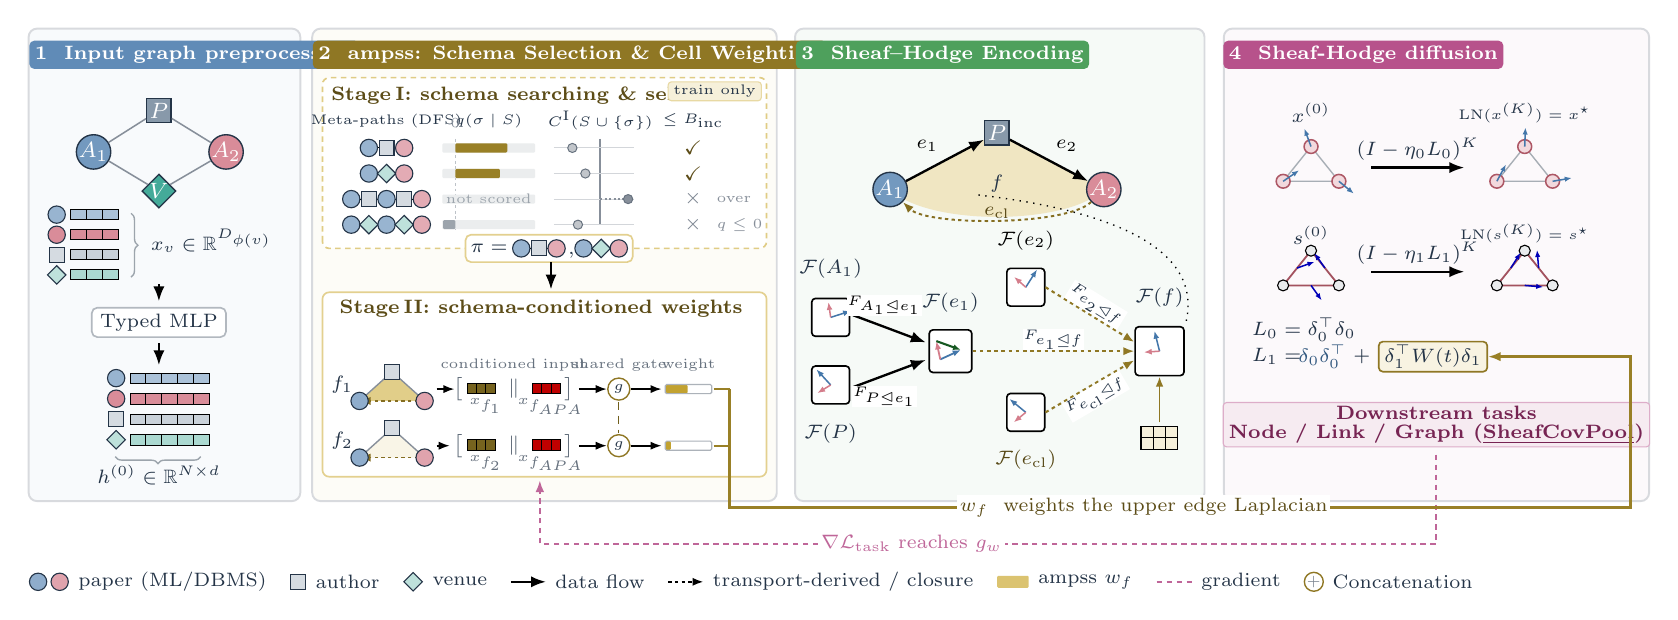
\begin{tikzpicture}[
  x=1.18cm,y=1.16cm,font=\footnotesize,text=ink,>=Latex,
  flow/.style     ={-{Latex[length=1.9mm]},line width=.85pt,draw=black},
  tflow/.style    ={-{Latex[length=1.4mm]},line width=.6pt,draw=black},
  derived/.style  ={-{Latex[length=1.4mm]},line width=.6pt,draw=black,
                    dash pattern=on 1.2pt off 1.2pt},
  lead/.style     ={dotted,draw=black,line width=.5pt},
  panel/.style    ={rounded corners=3pt,draw=ink!18,line width=.7pt},
  chip/.style     ={rounded corners=1.8pt,inner sep=2pt,font=\scriptsize\bfseries,
                    text=white,anchor=west},
  tag/.style      ={rounded corners=1.2pt,inner xsep=2pt,inner ysep=1.2pt,
                    font=\scriptsize,draw=ink!22,fill=white},
  nA/.style       ={circle,draw=ink,line width=.5pt,minimum size=3.6mm,inner sep=0, text=white},
  nP/.style       ={rectangle,draw=ink,line width=.5pt,minimum size=3.1mm,
                    inner sep=0,fill=cP!100, text=white},
  nV/.style       ={diamond,draw=ink,line width=.5pt,minimum width=3.8mm,
                    minimum height=3.8mm,inner sep=0,fill=cV!100, text=white},
  tP/.style       ={circle,draw=ink,line width=.4pt,minimum size=2.2mm,inner sep=0},
  tA/.style       ={rectangle,draw=ink,line width=.4pt,minimum size=1.9mm,
                    inner sep=0,fill=cP!35},
  tV/.style       ={diamond,draw=ink,line width=.4pt,minimum width=2.4mm,
                    minimum height=2.4mm,inner sep=0,fill=cV!35},
  stalk/.style    ={rounded corners=1.3pt,draw=black,line width=.6pt,fill=white,
                    minimum size=6.6mm,inner sep=0},
  taskbox/.style  ={rectangle,draw=ink!42,line width=.6pt,fill=white,
                    minimum width=1.48cm,minimum height=1.00cm,inner sep=1.5pt,
                    font=\tiny,align=center},
]

% ---------------- reusable drawing primitives ----------------
% ---- panel 2 carries three quantities that are NOT commensurable, so
% ---- each one gets its own mark; a bar never means two things here.
%   q      : signed, unbounded reward, composed of two terms -> BAR
%   C^I    : a position on a shared budget axis           -> MARKER
%   gates  : a fraction of 1                              -> CAPSULE
\newcommand{\rbar}[4]{\fill[#4,rounded corners=.4pt] (#1,#2) rectangle ++(#3,.10);}
\newcommand{\rtrack}[3]{\fill[ink!9,rounded corners=.4pt] (#1,#2) rectangle ++(#3,.10);}
% A stacked score bar: the whole length is q, and the dark head is the
% probe term, so `q = Delta_task + lambda Delta_cov' is read off the bar
% instead of stated beside it.  Drawn total-then-head so only the outer
% ends are rounded.  #1,#2 = zero-line origin, #3 = task, #4 = coverage.
\newcommand{\qbar}[4]{%
  \fill[gold!40,rounded corners=.4pt]      (#1,#2) rectangle ++(#3+#4,.10);
  \fill[gold!85!black,rounded corners=.4pt](#1,#2) rectangle ++(#3,.10);}
% C^I(S u {sigma}) is a cumulative subset cost tested against B_inc --
% four filled bars would read as four independent per-schema amounts,
% which is exactly what it is not.  A dot on a per-row rule reads as a
% position on a scale, and the B_inc rule is the thing it is tested
% against.  #1,#2 = axis left end.
\newcommand{\costaxis}[2]{\draw[ink!20,line width=.4pt] (#1,#2)--++(.86,0);}
\newcommand{\costdot}[3]{%
  \filldraw[fill=#3,draw=ink!70,line width=.35pt] (#1,#2) circle (.05);}
% A gate in [0,1].  The capsule outline IS the full scale, so a short
% fill reads as "this gate is nearly shut" rather than as a small
% amount of an unbounded quantity.  #3 = value in [0,1].
\newcommand{\gpillw}{.50}
\newcommand{\gpill}[4]{%
  \fill[#4,rounded corners=.5pt] (#1,#2) rectangle ++(#3*\gpillw,.10);
  \draw[ink!38,rounded corners=.5pt,line width=.4pt]
        (#1,#2) rectangle ++(\gpillw,.10);}
% Inline colour swatch, for keying a symbol in a label to a drawn bar.
% Explicit pt keeps it independent of the picture's x/y unit vectors.
\newcommand{\sw}[1]{\tikz[baseline=-.35ex]\fill[#1,rounded corners=.15pt]
  (0,0) rectangle (3.2pt,3.2pt);}
\newcommand{\lframe}[2]{%
  \draw[-{Latex[length=1.0mm]},cA,line width=.55pt]      (#1) -- ++(#2:.23);
  \draw[-{Latex[length=1.0mm]},cB!85,line width=.55pt]   (#1) -- ++({#2+80}:.17);}
\newcommand{\lframes}[2]{%
  \draw[-{Latex[length=.9mm]},cA,line width=.5pt]        (#1) -- ++(#2:.17);
  \draw[-{Latex[length=.9mm]},cB!85,line width=.5pt]     (#1) -- ++({#2+80}:.13);}
\newcommand{\chAPA}[2]{\draw[black,line width=.4pt](#1,#2)--++(.38,0);
  \node[tP,fill=cA!55]at(#1,#2){};\node[tA]at(#1+.19,#2){};
  \node[tP,fill=cB!55]at(#1+.38,#2){};}
\newcommand{\chAVA}[2]{\draw[black,line width=.4pt](#1,#2)--++(.38,0);
  \node[tP,fill=cA!55]at(#1,#2){};\node[tV]at(#1+.19,#2){};
  \node[tP,fill=cB!55]at(#1+.38,#2){};}
\newcommand{\chAPV}[2]{\draw[black,line width=.4pt](#1,#2)--++(.38,0);
  \node[tP,fill=cA!55]at(#1,#2){};\node[tA]at(#1+.19,#2){};
  \node[tV]at(#1+.38,#2){};}
\newcommand{\chAPAPA}[2]{\draw[black,line width=.4pt](#1,#2)--++(.76,0);
  \node[tP,fill=cA!55]at(#1,#2){};\node[tA]at(#1+.19,#2){};
  \node[tP,fill=cA!55]at(#1+.38,#2){};\node[tA]at(#1+.57,#2){};
  \node[tP,fill=cB!55]at(#1+.76,#2){};}
\newcommand{\chAVAVA}[2]{\draw[black,line width=.4pt](#1,#2)--++(.76,0);
  \node[tP,fill=cA!55]at(#1,#2){};\node[tV]at(#1+.19,#2){};
  \node[tP,fill=cA!55]at(#1+.38,#2){};\node[tV]at(#1+.57,#2){};
  \node[tP,fill=cB!55]at(#1+.76,#2){};}
\newcommand{\faceinst}[3]{%
  \fill[#3] (#1-.35,#2-.13) -- (#1,#2+.19) -- (#1+.35,#2-.13) -- cycle;
  \draw[ink!55,line width=.5pt] (#1-.35,#2-.13) -- (#1,#2+.19) -- (#1+.35,#2-.13);
  \draw[derived,draw=gold!65!black] (#1+.35,#2-.13) -- (#1-.35,#2-.13);
  \node[tP,fill=cA!60] at (#1-.35,#2-.13) {};
  \node[tA]            at (#1,#2+.19) {};
  \node[tP,fill=cB!60] at (#1+.35,#2-.13) {};}
\newcommand{\mgnodes}[4]{%
  \coordinate(q1)at($#1+(-.30,-.15)$);
  \coordinate(q2)at($#1+(0,.23)$);
  \coordinate(q3)at($#1+(.30,-.15)$);

  \draw[ink!40,line width=.5pt]
        (q1)--(q2)--(q3)--(q1);

  \foreach \p/\a in {q1/#2,q2/#3,q3/#4}{
    \filldraw[
      fill=cB!25,
      draw=cB!85!black,
      line width=.55pt
    ] (\p) circle (.075);

    \draw[
      -{Latex[length=.9mm]},
      cA,
      line width=.55pt
    ] (\p)--++(\a:.21);
  }
}
\newcommand{\mgedges}[4]{%
  \coordinate(q1)at($#1+(-.30,-.15)$);
  \coordinate(q2)at($#1+(0,.23)$);
  \coordinate(q3)at($#1+(.30,-.15)$);

  \draw[
    cB!80!black,
    line width=.65pt
  ] (q1)--(q2)--(q3)--(q1);

  \foreach \p in {q1,q2,q3}{
    \filldraw[
      fill=ink!10,
      draw=black,
      line width=.4pt
    ] (\p) circle (.06);
  }

  \foreach \p/\r/\a in {q1/q2/#2,q2/q3/#3,q3/q1/#4}{
    \coordinate(qm)at($(\p)!.5!(\r)$);

    \draw[
      -{Latex[length=.9mm]},
      blue!72!black,
      line width=.55pt
    ] (qm)--++(\a:.20);
  }
}
\newcommand{\embedding}[4]{%
  % #1 = start x
  % #2 = start y
  % #3 = fill color
  % #4 = number of bars (default = 3)
  \foreach \i in {1,...,#4}{
    \draw[
      draw=black,
      fill=#3,
      line width=.35pt
    ]
    ({#1 + .17*(\i-1)},#2)
    rectangle
    ({#1 + .17*\i},{#2 + .115});
  }
}
\newcommand{\embeddingsmall}[5]{%
  % #1 = start x
  % #2 = start y
  % #3 = fill color
  % #4 = number of bars (default = 3)
  % #5 = bar width (default = .17)
  \foreach \i in {1,...,#4}{
    \draw[
      draw=black,
      fill=#3,
      line width=.35pt
    ]
    ({#1 + #5*(\i-1)},#2)
    rectangle
    ({#1 + #5*\i},{#2 + .115});
  }
}
% =====================================================================
%  PANEL ORIGINS -- the only page-absolute numbers left in the figure.
%  Everything below is `\pNX`/`\pNY` plus a small local offset.
% =====================================================================
\pgfmathsetmacro{\pOneX}{1.56}    \pgfmathsetmacro{\pOneY}{3.39}
\pgfmathsetmacro{\pTwoX}{\pOneX+4.09}   \pgfmathsetmacro{\pTwoY}{\pOneY}
\pgfmathsetmacro{\pThreeX}{\pTwoX+4.90} \pgfmathsetmacro{\pThreeY}{\pTwoY}
\pgfmathsetmacro{\pFourX}{\pThreeX+4.70}\pgfmathsetmacro{\pFourY}{\pThreeY}
\coordinate (panel1-c) at (\pOneX,\pOneY);
\coordinate (panel2-c) at (\pTwoX,\pTwoY);
\coordinate (panel3-c) at (\pThreeX,\pThreeY);
\coordinate (panel4-c) at (\pFourX,\pFourY);

% =====================================================================
%  PANEL BACKGROUNDS
% =====================================================================
\node[panel,fill=cA!4,  minimum width=3.45cm,minimum height=6cm] at (panel1-c){};
\node[panel,fill=gold!4,minimum width=5.90cm,minimum height=6cm] at (panel2-c){};
\node[panel,fill=grn!4, minimum width=5.20cm,minimum height=6cm] at (panel3-c){};
\node[panel,fill=rose!3,minimum width=5.40cm,minimum height=6cm] at (panel4-c){};

\node[chip,fill=cA!85]         at (\pOneX-1.46,\pOneY+2.3)   {1\ \ Input graph preprocessing};
\node[chip,fill=gold!70!black] at (\pTwoX-2.5,\pTwoY+2.3)
      {2\ \ \textsc{ampss}: Schema Selection \& Cell Weighting};
\node[chip,fill=grn!80]        at (\pThreeX-2.2,\pThreeY+2.3){3\ \ Sheaf--Hodge Encoding};
\node[chip,fill=rose!85]       at (\pFourX-2.3,\pFourY+2.3) {4\ \ Sheaf-Hodge diffusion};

% =====================================================================
%  PANEL 1 -- typed input, unequal features -> shared stalk R^d
%
%  Global vertical adjustment:
%    \pOneContentDY > 0  moves all Panel-1 content upward.
%    \pOneContentDY < 0  moves all Panel-1 content downward.
%
%  The panel background and title chip are not shifted.
% =====================================================================

\pgfmathsetmacro{\pOneContentDY}{0.1}

\begin{scope}[shift={(0,\pOneContentDY)}]

% ---------------------------------------------------------------------
% Typed input graph
% ---------------------------------------------------------------------
\node[nP]
      (p1)
      at (\pOneX-.06,\pOneY+1.59)
      {$P$};

\node[nA,fill=cA!75]
      (a1)
      [below left=.2017cm and .5053cm of p1]
      {$A_{1}$};

\node[nA,fill=cB!75]
      (a2)
      [below right=.2017cm and .5289cm of p1]
      {$A_{2}$};

\node[nV]
      (v1)
      [below=.6350cm of p1]
      {$V$};

\foreach \s/\t in {a1/p1,p1/a2,a1/v1,v1/a2}{
  \draw[ink!55,line width=.55pt]
        (\s)--(\t);
}
% ---------------------------------------------------------------------
% Type-dependent input features
% ---------------------------------------------------------------------
\pgfmathsetmacro{\typelegdy}{.22}

% Paper, class 1
\node[tP,fill=cA!55]
      at (\pOneX-1.16,\pOneY+.45)
      {};

\embedding
  {\pOneX-1.01}
  {\pOneY+.395}
  {cA!45}
  {3}

% Paper, class 2
\node[tP,fill=cB!75]
      at (\pOneX-1.16,\pOneY+.45-\typelegdy)
      {};

\embedding
  {\pOneX-1.01}
  {\pOneY+.395-\typelegdy}
  {cB!75}
  {3}

% Author
\node[tA]
      at (\pOneX-1.16,\pOneY+.45-2*\typelegdy)
      {};

\embedding
  {\pOneX-1.01}
  {\pOneY+.395-2*\typelegdy}
  {cP!45}
  {3}

% Venue
\node[tV]
      at (\pOneX-1.16,\pOneY+.45-3*\typelegdy)
      {};

\embedding
  {\pOneX-1.01}
  {\pOneY+.395-3*\typelegdy}
  {cV!45}
  {3}

% Group the heterogeneous input features.
\draw[
  decorate,
  decoration={
    brace,
    mirror,
    amplitude=2.5pt
  },
  ink!45,
  line width=.5pt
]
  (\pOneX-.36,\pOneY-.235)
  --
  (\pOneX-.36,\pOneY+.465);

% Input-feature notation
\node[
  font=\scriptsize,
  anchor=west
]
  (xv)
  at (\pOneX-.25,\pOneY+.16)
  {$x_v\in\mathbb{R}^{D_{\phi(v)}}$};

% Data-flow origin below the input-feature block
\coordinate
  (xvFlow)
  at (\pOneX-.06,\pOneY-.28);

% ---------------------------------------------------------------------
% Type-specific encoder
% ---------------------------------------------------------------------
\node[
  rounded corners=2pt,
  draw=ink!35,
  fill=white,
  line width=.6pt,
  inner xsep=3pt,
  inner ysep=2.2pt,
  font=\scriptsize
]
  (enc)
  at (\pOneX-.06,\pOneY-.73)
  {Typed MLP};

\draw[
  flow,
  shorten <=1pt,
  shorten >=2pt
]
  (xvFlow)
  --
  (enc.north);

% Optional equation reference
% \node[
%   anchor=west,
%   fill=white,
%   inner sep=.6pt
% ]
%   at (\pOneX+.62,\pOneY-.75)
%   {\eqn{eq:node-encoder}};

% ---------------------------------------------------------------------
% Shared d-dimensional node stalks
% ---------------------------------------------------------------------
\coordinate
  (hzeroTop)
  at (\pOneX-.06,\pOneY-1.26);

\draw[
  flow,
  shorten <=2pt,
  shorten >=2pt
]
  (enc.south)
  --
  (hzeroTop);

\pgfmathsetmacro{\hzerody}{.15}

% Paper, class 1
\node[tP,fill=cA!55]
      at (\pOneX-.52,\pOneY-1.34)
      {};

\embedding
  {\pOneX-.37}
  {\pOneY-1.40}
  {cA!45}
  {5}

% Paper, class 2
\node[tP,fill=cB!75]
      at (\pOneX-.52,\pOneY-1.34-1.5*\hzerody)
      {};

\embedding
  {\pOneX-.37}
  {\pOneY-1.40-1.5*\hzerody}
  {cB!75}
  {5}

% Author
\node[tA]
      at (\pOneX-.52,\pOneY-1.34-3*\hzerody)
      {};

\embedding
  {\pOneX-.37}
  {\pOneY-1.40-3*\hzerody}
  {cP!45}
  {5}

% Venue
\node[tV]
      at (\pOneX-.52,\pOneY-1.34-4.5*\hzerody)
      {};

\embedding
  {\pOneX-.37}
  {\pOneY-1.40-4.5*\hzerody}
  {cV!45}
  {5}

% Group the encoded node representations.
\draw[
  decorate,
  decoration={
    brace,
    mirror,
    amplitude=2.5pt
  },
  ink!45,
  line width=.5pt
]
  (\pOneX-.53,\pOneY-2.20)
  --
  (\pOneX+.39,\pOneY-2.20);

\node[
  font=\scriptsize
]
  at (\pOneX-.06,\pOneY-2.40)
  {$h^{(0)}\in\mathbb{R}^{N\times d}$};

\end{scope}

% =====================================================================
%  PANEL 2 -- AMPSS
%  Stage I is a CANDIDATE TABLE, one row per schema:
%      [typed-path glyph | held-out task-gain bar | C^I marker
%       on a shared axis vs the B_inc rule | keep/drop | reason]
%  so both rejection modes of `src/data/stage1_selector.py` are drawn as
%  geometry rather than asserted in text: a bar left of the 0 rule
%  (nonpositive marginal gain) and a marker past the B_inc rule.  A
%  budget-infeasible candidate is skipped BEFORE the probe is fitted, so
%  that row deliberately carries no q bar at all.
%  Every label in the header band sits on ONE line -- stacking a rule
%  label under a column name is what made this band read as crowded.
%  The Sigma chip straddles the Stage-I frame: it is literally what
%  Stage I emits and what Stage II weights.
% =====================================================================
% ---- column geometry: one macro per column, reused by all four rows --
\pgfmathsetmacro{\sIgx}{\pTwoX-1.7}    % candidate glyph centre
\pgfmathsetmacro{\sIql}{\pTwoX-1.10}    % q track, left edge (width 1.00)
\pgfmathsetmacro{\sIqz}{\pTwoX-0.96}    % q = 0 rule
\pgfmathsetmacro{\sIcl}{\pTwoX+0.1}    % cumulative incidence axis
\pgfmathsetmacro{\sIbx}{\pTwoX+0.6}    % B_inc threshold
\pgfmathsetmacro{\sImk}{\pTwoX+1.6}    % keep / drop mark
\pgfmathsetmacro{\sIry}{\pTwoY+1.28}    % first candidate row
\pgfmathsetmacro{\stageIdy}{.28}        % row step, reused 4x

\draw[rounded corners=2.5pt,draw=gold!60,line width=.6pt,fill=white,
      dash pattern=on 2pt off 1.6pt]
      (\pTwoX-2.39,\pTwoY+.18) rectangle (\pTwoX+2.39,\pTwoY+2.05);
\node[font=\scriptsize\bfseries,text=gold!45!black,anchor=west]
      at (\pTwoX-2.4,\pTwoY+1.85){Stage\,I: schema searching \& selection};
\node[tag,font=\tiny,fill=gold!18,draw=gold!45,anchor=east]
      at (\pTwoX+2.34,\pTwoY+1.9){train only};

% Stage-I columns: candidate schema, selection gain, budget feasibility,
% and the resulting keep/drop decision.
\node[font=\tiny]
      at (\sIgx+.0,\pTwoY+1.58)
      {Meta-paths (DFS)};

\node[font=\tiny]
      at (\sIql+.50,\pTwoY+1.58)
      {$q(\sigma\mid S)$};

\node[font=\tiny,align=center]
      at (\sIcl+0.5,\pTwoY+1.58)
      {$C^{\mathrm I}(S\cup\{\sigma\})$};
\node[font=\tiny,align=center]
      at (\sImk+0,\pTwoY+1.58)
      {$\leq B_{\mathrm{inc}}$};

% The dashed rule is q=0; the solid rule is the incidence threshold.
\node[font=\tiny,text=ink!55,anchor=south]
      at (\sIqz,\pTwoY+1.40){$0$};

\draw[ink!30,line width=.45pt,dash pattern=on 1pt off 1pt]
      (\sIqz,\pTwoY+1.38) -- (\sIqz,\pTwoY+.37);

\draw[ink!55,line width=.55pt]
      (\sIbx,\pTwoY+1.38) -- (\sIbx,\pTwoY+.44);

% row 1 -- accepted: large probe gain
\chAPA{\sIgx-.19}{\sIry}
\rtrack{\sIql}{\sIry-.05}{1.00}
\rbar{\sIqz}{\sIry-.05}{.56}{gold!75!black}
\costaxis{\sIcl}{\sIry}  \costdot{\sIcl+.20}{\sIry}{ink!28}
\node[font=\scriptsize,text=gold!45!black] at (\sImk,\sIry){$\checkmark$};

% row 2 -- accepted: smaller but positive held-out task gain
\chAVA{\sIgx-.19}{\sIry-\stageIdy}
\rtrack{\sIql}{\sIry-\stageIdy-.05}{1.00}
\rbar{\sIqz}{\sIry-\stageIdy-.05}{.48}{gold!75!black}
\costaxis{\sIcl}{\sIry-\stageIdy}  \costdot{\sIcl+.34}{\sIry-\stageIdy}{ink!28}
\node[font=\scriptsize,text=gold!45!black] at (\sImk,\sIry-\stageIdy){$\checkmark$};

% row 3 -- infeasible: the trial subset overruns B_inc, so it is never
% scored (the selector `continue`s before fitting the probe)
\chAPAPA{\sIgx-.38}{\sIry-2*\stageIdy}
\rtrack{\sIql}{\sIry-2*\stageIdy-.05}{1.00};
\node[font=\tiny,text=ink!45] at (\sIql+.50,\sIry-2*\stageIdy){not scored};
\costaxis{\sIcl}{\sIry-2*\stageIdy}
\draw[ink!55,line width=.5pt,dash pattern=on .8pt off .8pt]
      (\sIbx,\sIry-2*\stageIdy) -- (\sIcl+.80,\sIry-2*\stageIdy);
\costdot{\sIcl+.80}{\sIry-2*\stageIdy}{ink!55}
\node[font=\scriptsize,text=ink!60] at (\sImk,\sIry-2*\stageIdy){$\times$};
\node[font=\tiny,text=ink!55,anchor=west]
      at (\sImk+.15,\sIry-2*\stageIdy){over};

% row 4 -- feasible but the marginal gain is nonpositive
\chAVAVA{\sIgx-.38}{\sIry-3*\stageIdy}
\rtrack{\sIql}{\sIry-3*\stageIdy-.05}{1.00};
\rbar{\sIqz-.13}{\sIry-3*\stageIdy-.05}{.13}{ink!45};
\costaxis{\sIcl}{\sIry-3*\stageIdy}  \costdot{\sIcl+.26}{\sIry-3*\stageIdy}{ink!28}
\node[font=\scriptsize,text=ink!60] at (\sImk,\sIry-3*\stageIdy){$\times$};
\node[font=\tiny,text=ink!55,anchor=west]
      at (\sImk+.15,\sIry-3*\stageIdy){$q\leq0$};

% the selected pool: drawn straddling the frame, i.e. the interface
\draw[rounded corners=2pt,draw=gold!55,line width=.6pt,fill=white]
      (\pTwoX-.85,\pTwoY+.03) rectangle (\pTwoX+.95,\pTwoY+.33);
\node[font=\scriptsize,anchor=west] at (\pTwoX-.9,\pTwoY+.18){$\pi=$};
\chAPA{\pTwoX-.25}{\pTwoY+.18}; 
\node[font=\scriptsize,anchor=west] at (\pTwoX+0.15,\pTwoY+.1){$,$};
\chAVA{\pTwoX+.42}{\pTwoY+.18};

\draw[flow,shorten >=1pt] (\pTwoX+.07,\pTwoY+.03) -- (\pTwoX+.07,\pTwoY-.30);

% ---------------------------------------------------------------------
%  Stage II. Each retained path instance receives one task-learned
%  weight conditioned on both its ordered path latent z_f and the
%  embedding e_{sigma(f)} of its selected schema. The two rows belong
%  to the same schema, showing instance-level variation without a
%  separate multiplicative schema gate.
% ---------------------------------------------------------------------
\pgfmathsetmacro{\sIIsy}{\pTwoY-0.90}     % weighting equation
\pgfmathsetmacro{\sIIry}{\pTwoY-1.36}     % instance row 1
\pgfmathsetmacro{\stageIIdy}{.42}         % row step, reused 2x
\pgfmathsetmacro{\sIIfx}{\pTwoX-1.64}     % face-instance centre
\pgfmathsetmacro{\sIIbl}{\pTwoX-0.98}     % conditioned input capsule
\pgfmathsetmacro{\sIIax}{\pTwoX+0.8}     % shared weighting network
\pgfmathsetmacro{\sIIwl}{\pTwoX+1.3}     % w_f capsule, left edge
\pgfmathsetmacro{\sIIbus}{\pTwoX+2}    % collector bus out of panel

\draw[rounded corners=2.5pt,draw=gold!55,line width=.6pt,fill=white]
      (\pTwoX-2.39,\pTwoY-2.32) rectangle (\pTwoX+2.39,\pTwoY-.30);
\node[font=\scriptsize\bfseries,text=gold!45!black,anchor=west]
      at (\pTwoX-2.31,\pTwoY-.48)
      {Stage\,II: schema-conditioned weights};

% A single learned weight replaces the former schema--instance product.
%\node[font=\tiny,align=center,text=black!75]
%      at (\pTwoX,\sIIsy+0.1)
%      {$w_f(t)=(1-r(t))+2r(t)\,
%        \operatorname{sigmoid}\!\bigl(g_w(z_f\mathbin\Vert e_{\sigma(f)})\bigr)$};

% Compact visual headings; keep the original column coordinates.

\node[font=\tiny,text=ink!70]
      at (\sIIbl+0.65,\pTwoY-1.10) {conditioned input};

\node[font=\tiny,text=ink!70]
      at (\sIIax,\pTwoY-1.10) {shared gate};
\node[font=\tiny,text=ink!70]
      at (\sIIwl+.25,\pTwoY-1.10) {weight};

% Dashed tie indicates that both rows use the same g_w.
% Draw it before the white gate nodes so it does not cross their interiors.
\draw[gold!55!black,densely dashed,line width=.4pt]
      (\sIIax,\sIIry-.14)
      -- (\sIIax,\sIIry-\stageIIdy-.06);

% ---------------------------------------------------------------------
% Instance row 1 -- strongly weighted APA occurrence
% ---------------------------------------------------------------------
\faceinst{\sIIfx}{\sIIry}{gold!58};
\node[font=\scriptsize,anchor=west]
      at (\pTwoX-2.40,\sIIry+.05) {$f_1$};

\draw[tflow]
      (\sIIfx+.48,\sIIry) -- (\sIIbl-.04+0.05,\sIIry);


% [.
\node[font=\scriptsize,text=ink!75] at (\sIIbl+0.05,\sIIry) {$\bigl[$};

 
% Ordered path latent z_{f_1}: segmented feature strip.
\embeddingsmall{\sIIbl+0.15}{\sIIry-.05}{gold!58!black}{3}{0.1}

\node[font=\fontsize{4.5pt}{5pt}\selectfont,text=ink!70]
      at (\sIIbl+.35,\pTwoY-1.55) {$x_{f_{1}}$};
      
% Concatenation operator.
\node[font=\scriptsize,text=ink!75]
      at (\sIIbl+0.65,\sIIry) {$\Vert$};

% Learned embedding e_APA: same strip in both rows.
\embeddingsmall{\sIIbl+0.85}{\sIIry-.05}{red!75!black}{3}{0.1};

\node[font=\fontsize{4.5pt}{5pt}\selectfont,text=ink!70]
      at (\sIIbl+1.05,\pTwoY-1.55) {$x_{f_{APA}}$};

% ].
\node[font=\scriptsize,text=ink!75] at (\sIIbl+1.2+0.05,\sIIry) {$\bigr]$};

\draw[tflow]
      (\sIIbl+1.35,\sIIry) -- (\sIIax-.13,\sIIry);

\node[circle,draw=gold!70!black,fill=white,line width=.5pt,
      minimum size=2.8mm,inner sep=0,font=\tiny]
      at (\sIIax,\sIIry) {$g$};

\draw[tflow]
      (\sIIax+.13,\sIIry) -- (\sIIwl-.04,\sIIry);
\gpill{\sIIwl}{\sIIry-.05}{.48}{gold!95!black}

% ---------------------------------------------------------------------
% Instance row 2 -- suppressed occurrence of the same APA schema
% ---------------------------------------------------------------------
\faceinst{\sIIfx}{\sIIry-\stageIIdy-.20}{gold!12};
\node[font=\scriptsize,anchor=west]
      at (\pTwoX-2.40,\sIIry-\stageIIdy-.15) {$f_2$};

\draw[tflow]
      (\sIIfx+.48,\sIIry-\stageIIdy-.20)
      -- (\sIIbl-.04,\sIIry-\stageIIdy-.20);

% [.
\node[font=\scriptsize,text=ink!75] at (\sIIbl+0.05,\sIIry-\stageIIdy-.20) {$\bigl[$};

 
% Ordered path latent z_{f_1}: segmented feature strip.
\embeddingsmall{\sIIbl+0.15}{\sIIry-.05-\stageIIdy-0.2}{gold!58!black}{3}{0.1}

\node[font=\fontsize{4.5pt}{5pt}\selectfont,text=ink!70]
      at (\sIIbl+.35,\pTwoY-1.55-\stageIIdy-0.2) {$x_{f_{2}}$};
      
% Concatenation operator.
\node[font=\scriptsize,text=ink!75]
      at (\sIIbl+0.65,\sIIry-\stageIIdy-.20) {$\Vert$};

% Learned embedding e_APA: same strip in both rows.
\embeddingsmall{\sIIbl+0.85}{\sIIry-.05-\stageIIdy-0.2}{red!75!black}{3}{0.1};

\node[font=\fontsize{4.5pt}{5pt}\selectfont,text=ink!70]
      at (\sIIbl+1.05,\pTwoY-1.55-\stageIIdy-0.2) {$x_{f_{APA}}$};

% ].
\node[font=\scriptsize,text=ink!75] at (\sIIbl+1.2+0.05,\sIIry-\stageIIdy-0.2) {$\bigr]$};


\draw[tflow]
      (\sIIbl+1.35,\sIIry-\stageIIdy-.20) -- (\sIIax-.13,\sIIry-\stageIIdy-.20);

\node[circle,draw=gold!70!black,fill=white,line width=.5pt,
      minimum size=2.8mm,inner sep=0,font=\tiny]
      at (\sIIax,\sIIry-\stageIIdy-.20) {$g$};

\draw[tflow]
      (\sIIax+.13,\sIIry-\stageIIdy-.20)
      -- (\sIIwl-.04,\sIIry-\stageIIdy-.20);
\gpill{\sIIwl}{\sIIry-\stageIIdy-.25}{.12}{gold!95!black}

% Both instance weights leave the panel on the original collector bus.
\draw[gold!75!black,line width=.7pt]
      (\sIIwl+.52,\sIIry) -- (\sIIbus,\sIIry);
\draw[gold!75!black,line width=.7pt]
      (\sIIwl+.52,\sIIry-\stageIIdy-0.2) -- (\sIIbus,\sIIry-\stageIIdy-0.2);

% =====================================================================
%  PANEL 3 -- one closed path support and its cellular-sheaf maps
% =====================================================================
\coordinate (fa1) at (\pThreeX-1.65+0.47,\pThreeY+.825);
\coordinate (fp1) at (\pThreeX-.5+0.47, \pThreeY+1.445);
\coordinate (fa2) at (\pThreeX+.65+0.47,\pThreeY+.825);
\fill[gold!30] (fa1) -- (fp1) -- (fa2)
   .. controls (\pThreeX+.25+0.47,\pThreeY+.425) and (\pThreeX-1.25+0.47,\pThreeY+.425) .. (fa1) -- cycle;
\node[nA,fill=cA!75] (F1) at (fa1){$A_1$};
\node[nP]            (F2) at (fp1){$P$};
\node[nA,fill=cB!75] (F3) at (fa2){$A_2$};
\draw[flow] (F1)--(F2);  \draw[flow] (F2)--(F3);
\draw[derived,draw=gold!65!black,line width=.7pt]
      (F3) .. controls (\pThreeX+.25+0.47,\pThreeY+.425) and (\pThreeX-1.25+0.47,\pThreeY+.425) .. (F1);
\node[font=\scriptsize,text=black] at (\pThreeX-1.25+0.47,\pThreeY+1.305){$e_1$};
\node[font=\scriptsize,text=black] at (\pThreeX+.25+0.47, \pThreeY+1.305){$e_2$};
\node[font=\scriptsize,text=gold!42!black] at (\pThreeX-.5+0.47,\pThreeY+.565){$e_{\mathrm{cl}}$};
\node[font=\scriptsize] at (\pThreeX-.5+0.47,\pThreeY+.885){$f$};

% One observed boundary edge is expanded at left: its two endpoint
% restrictions point in the cellular-sheaf direction, node -> edge.
\node[stalk,minimum size=4.8mm] (su) at (\pThreeX-1.82,\pThreeY-.575){};
\node[stalk,minimum size=4.8mm] (sv) at (\pThreeX-1.82,\pThreeY-1.315){};
\node[stalk,minimum size=5.4mm] (se1) at (\pThreeX-.53,\pThreeY-.945){};
\lframe{su.center}{18};
\lframe{sv.center}{132};

\node[font=\scriptsize,anchor=south] at (\pThreeX-1.82,\pThreeY-.255){$\mathcal F(A_1)$};
\node[font=\scriptsize,anchor=north] at (\pThreeX-1.82,\pThreeY-1.635){$\mathcal F(P)$};
\node[font=\scriptsize,anchor=south] at (\pThreeX-.53,\pThreeY-.625){$\mathcal F(e_1)$};

% Each node--edge incidence is shown in both operator directions:
% the restriction F enters delta_0, while F^T is its adjoint.
\draw[flow,shorten <=1pt,shorten >=1pt]
      ($(su.east)+(0,.035)$) -- ($(se1.west)+(0,.085)$);

\draw[flow,shorten <=1pt,shorten >=1pt]
      ($(sv.east)+(0,-.035)$) -- ($(se1.west)+(0,-.085)$);

\node[font=\tiny,fill=white,inner sep=.35pt,anchor=south,text=black]
      at (\pThreeX-1.24,\pThreeY-.565){$F_{A_1\unlhd e_1}$};
\node[font=\tiny,fill=white,inner sep=.35pt,anchor=north,text=black]
      at (\pThreeX-1.24,\pThreeY-1.325){$F_{P\unlhd e_1}$};

%      \node[font=\tiny,text=black,anchor=north]
%     at (\pThreeX-1.06,\pThreeY-1.805)
%     {$\Phi(h_{A_1}^{(0)},h_P^{(0)},z_{r_1})$\,\eqn{eq:conformal-map}};

% The two transported endpoint vectors and their oriented difference
% live in the same edge stalk.
\draw[-{Latex[length=1.05mm]},cA,line width=.65pt]
      ($(se1.center)+(-.11,-.09)$)--++(25:.245);
\draw[-{Latex[length=1.05mm]},cB!85,line width=.65pt]
      ($(se1.center)+(-.11,-.09)$)--++(102:.205);
\draw[-{Latex[length=1.0mm]},grn!65!black,line width=.75pt]
      ($(se1.center)+(102:.205)+(-.11,-.09)$) --
      ($(se1.center)+(25:.245)+(-.11,-.09)$);
%\node[font=\tiny,text=grn!55!black,anchor=north]
%      at (\pThreeX-.53,\pThreeY-1.285)
%      {$(\delta_0x)_{e_1}$\,\eqn{eq:delta0}};

% The remaining boundary edge stalks.  All three maps terminate
% independently in one shared face stalk; there is deliberately no
% pooling junction.
\node[stalk,minimum size=4.8mm] (se2) at (\pThreeX+.28,\pThreeY-.245){};
\node[stalk,minimum size=4.8mm] (sec) at (\pThreeX+.28,\pThreeY-1.615){};
\node[stalk,minimum size=6.2mm] (sf)  at (\pThreeX+1.72,\pThreeY-.945){};
\lframe{se2.center}{58};
\lframe{sec.center}{140};
\lframe{sf.center}{104};

\node[font=\scriptsize,anchor=south,text=black]
      at (\pThreeX+.28,\pThreeY+.055){$\mathcal F(e_2)$};
\node[font=\scriptsize,anchor=north,text=gold!42!black]
      at (\pThreeX+.28,\pThreeY-1.915){$\mathcal F(e_{\mathrm{cl}})$};
\node[font=\scriptsize,anchor=south]
      at (\pThreeX+1.72,\pThreeY-.575){$\mathcal F(f)$};

\draw[-{Latex[length=1.4mm]},line width=.75pt,draw=gold!70!black,
      dash pattern=on 1.3pt off 1.3pt]
      (se1.east) --
      node[midway,above,font=\tiny,fill=white,inner sep=.4pt]
      {$F_{e_1\unlhd f}$} (sf.west);
\draw[-{Latex[length=1.4mm]},line width=.75pt,draw=gold!70!black,
      dash pattern=on 1.3pt off 1.3pt]
      (se2.east) --
      node[midway,above,sloped,font=\tiny,fill=white,inner sep=.4pt]
      {$F_{e_2\unlhd f}$}
      ($(sf.west)+(0,.10)$);

\draw[-{Latex[length=1.4mm]},line width=.75pt,draw=gold!70!black,
      dash pattern=on 1.3pt off 1.3pt]
      (sec.east) --
      node[midway,below,sloped,font=\tiny,fill=white,inner sep=.4pt]
      {$F_{e_{\mathrm{cl}}\unlhd f}$}
      ($(sf.west)+(0,-.10)$);

% A_f selects the common face frame from which the three incidence
% maps are transported; it is not a pooling operator.
\foreach \i in {0,1,2}\foreach \j in {0,1}{
  \draw[black,line width=.4pt,fill=gold!18]
        (\pThreeX+1.52+.13*\i,\pThreeY-2.025+.13*\j) rectangle ++(.13,.13);}
\draw[-{Latex[length=1.3mm]},line width=.65pt,draw=gold!70!black]
      (\pThreeX+1.72,\pThreeY-1.725)--(sf.south);
%\node[font=\scriptsize,anchor=west]
%      at (\pThreeX+1.52,\pThreeY-2.2){$A_f$\,\eqn{eq:face-map}};

% The drawn 2-cell and the shared face stalk are the same object.
\draw[lead] (\pThreeX-.23,\pThreeY+.765)
     .. controls (\pThreeX+1.25,\pThreeY+.59)
     and (\pThreeX+2.20,\pThreeY+.16) .. ($(sf)+(.28,.30)$);

% =====================================================================
%  PANEL 4 -- parallel diffusion + task heads
%  The x^(0)->x* and s^(0)->s* rows are `chains` (unchanged from the
%  previous pass); the task-head groups and their small decorations
%  are now off `\pFourX,\pFourY` the same way as the other panels.
% =====================================================================
\begin{scope}[start chain=xdiff going right, node distance=2.714cm]
\node[coordinate,on chain=xdiff] (x0)    at (\pFourX-1.35,\pFourY+1.065){};
\node[coordinate,on chain=xdiff] (xstar) {};
\end{scope}
\mgnodes{(x0)}{35}{110}{-40};
\mgnodes{(xstar)}{62}{ 88}{ 10};
\draw[flow] ($(x0)+(\gutter,0)$)--($(xstar)+(-\gutter,0)$);
\node[font=\scriptsize] at ($(x0)!.5!(xstar)+(0,.20)$){$(I-\eta_0L_0)^K$};
\node[font=\scriptsize] at ($(x0)+(0,.6)$){$x^{(0)}$};
\node[font=\tiny] at ($(xstar)+(0,.6)$){$\operatorname{LN}(x^{(K)})=x^{\star}$};

\begin{scope}[start chain=sdiff going right, node distance=2.714cm]
\node[coordinate,on chain=sdiff]
  (s0) at (\pFourX-1.35,\pFourY+0.425-0.5){};
\node[coordinate,on chain=sdiff] (sstar) {};
\end{scope}

\mgedges{(s0)}{20}{125}{-55};
\mgedges{(sstar)}{58}{95}{-5};

\draw[flow]
  ($(s0)+(\gutter,0)$)
  --
  ($(sstar)+(-\gutter,0)$);

\node[font=\scriptsize]
  at ($(s0)!.5!(sstar)+(0,.20)$)
  {$(I-\eta_1L_1)^K$};

\node[font=\scriptsize]
  at ($(s0)+(0,.40)$)
  {$s^{(0)}$};

\node[font=\tiny]
  at ($(sstar)+(0,.42)$)
  {$\operatorname{LN}(s^{(K)})=s^{\star}$};

%\node[anchor=west]
%  at ($(sstar)+(.56,.40)$)
%  {\eqn{eq:diffusion}};

\node[font=\scriptsize,anchor=west]
  at (\pFourX-2.09,\pFourY-.105-0.6)
  {$L_0=\delta_0^{\top}\delta_0$};

%\node[font=\scriptsize,anchor=west]
%  at (\pFourX-.30,\pFourY-.105-0.5)
%  {\eqn{eq:l0}};

\node[font=\scriptsize,anchor=west]
  at (\pFourX-2.09,\pFourY-.405-0.6)
  {$L_1=$};

\node[font=\scriptsize,anchor=west,text=cA!75!black]
  at (\pFourX-1.59,\pFourY-.405-0.6)
  {$\delta_0\delta_0^{\top}$};

\node[font=\scriptsize,anchor=west]
  at (\pFourX-1.0,\pFourY-.405-0.6)
  {$+$};

\node[
  rounded corners=1.5pt,
  draw=gold!70!black,
  fill=gold!14,
  line width=.6pt,
  inner xsep=2pt,
  inner ysep=1.2pt,
  font=\scriptsize,
  anchor=west
]
  (upperterm)
  at (\pFourX-.63,\pFourY-.405-0.6)
  {$\delta_1^{\top}W(t)\delta_1$};

%\node[font=\scriptsize,anchor=west]
%  at (\pFourX+1.16,\pFourY-.405-0.5)
%  {\eqn{eq:l1}};

% ---- one downstream-task block with the exact task-specific readouts ----
\node[tag,draw=rose!40,fill=rose!10,text=rose!70!black,
      font=\scriptsize\bfseries,align=center]
      (downstream) at (\pFourX,\pFourY0-1.75)
      {Downstream tasks\\[-1pt]
       \textsc{Node} / \textsc{Link} /
       \textsc{Graph (\underline{SheafCovPool})}};
% =====================================================================
%  WIRING -- face weights enter L_1; task gradients reach AMPSS gates
% =====================================================================
\coordinate (grad-start)
  at ($(downstream.south)+(0,-.08)$);
\coordinate (grad-baseline1)
  at (\pFourX,\pFourY-3.055);
\coordinate (grad-baseline2)
  at (\pTwoX-.05,\pTwoY-3.055);
\coordinate (grad-target)
  at (\pTwoX-.05,\pTwoY-2.36);
\coordinate (grad-label)
  at (\pThreeX-.95,\pThreeY-3.055);

% leaves on the w_f collector bus, at the same x as the two output gates
\coordinate (wf-source)
  at (\pTwoX+1.99,\pTwoY-1.36);
\coordinate (wf-baseline)
  at (\pTwoX+1.99,\pTwoY-2.655);
\coordinate (wf-riser)
  at (\pFourX+2.09,\pFourY-2.655);
\coordinate (wf-turn)
  at (\pFourX+2.09,\pFourY-.405-0.6);
\coordinate (wf-label)
  at (\pThreeX+1.55,\pThreeY-2.655);

% Task-loss gradient back to the AMPSS gates
\draw[-{Latex[length=1.5mm]},rose!75,line width=.7pt,
      dash pattern=on 2pt off 1.6pt]
  (grad-start)
  -- (grad-baseline1)
  -- (grad-baseline2)
  -- (grad-target);

\node[font=\scriptsize,text=rose!75,fill=white,inner sep=1pt]
  at (grad-label)
  {$\nabla\mathcal{L}_{\mathrm{task}}
    \textnormal{ reaches }
    g_w$};

% Face weights enter the weighted upper edge Laplacian
\draw[-{Latex[length=1.6mm]},gold!75!black,line width=.85pt]
  (wf-source)
  -- (wf-baseline)
  -- (wf-riser)
  -- (wf-turn)
  -- (upperterm.east);

\node[font=\scriptsize,text=gold!45!black,fill=white,inner sep=1pt]
  at (wf-label)
  {$w_f$ \textnormal{ weights the upper edge Laplacian}};

% =====================================================================
%  LEGEND -- a running chain of plain-number offsets: each item's x is
%  "previous item's x + this gap" via `\pgfmathsetmacro`, instead of a
%  row of independently typed absolute x-coordinates. (The `positioning`
%  library's own edge-to-edge gap semantics need a size-dependent
%  correction per node pair -- clean for the fixed-size markers used in
%  panel 1 / panel 3 above, but error-prone here where markers and
%  variable-width text labels alternate -- so the legend instead reuses
%  the same "origin + local offset" idiom as the rest of the figure.)
% =====================================================================
% Equal edge-to-edge spacing within and between legend groups.
\def\legendLabelGap{1.2mm} % image right edge -> label left edge
\def\legendGroupGap{3.0mm} % previous group right edge -> next group left edge

\begin{scope}[
  legendtext/.style={
    font=\scriptsize,
    inner sep=0pt,
    outer sep=0pt
  },
  legendfit/.style={
    inner sep=0pt,
    outer sep=0pt
  },
  legendline/.style={
    inner sep=0pt,
    outer sep=0pt,
    minimum width=.448cm, % .38 TikZ x-units at x=1.18cm
    minimum height=2.2mm
  }
]

% ---------------------------------------------------------------------
% Paper group
% ---------------------------------------------------------------------
\node[tP,fill=cA!60] (leg-paper-a) at (.20,-.08) {};

% Internal spacing between the two paper markers.
\node[tP,fill=cB!60,right=.40mm of leg-paper-a]
      (leg-paper-b) {};

\node[legendfit,fit=(leg-paper-a)(leg-paper-b)]
      (leg-paper-icon) {};

\node[legendtext,right=\legendLabelGap of leg-paper-icon]
      (leg-paper-text) {paper (ML/DBMS)};

\node[legendfit,fit=(leg-paper-icon)(leg-paper-text)]
      (leg-paper-group) {};

% ---------------------------------------------------------------------
% Author group
% ---------------------------------------------------------------------
\node[tA,right=\legendGroupGap of leg-paper-group]
      (leg-author-icon) {};

\node[legendtext,right=\legendLabelGap of leg-author-icon]
      (leg-author-text) {author};

\node[legendfit,fit=(leg-author-icon)(leg-author-text)]
      (leg-author-group) {};

% ---------------------------------------------------------------------
% Venue group
% ---------------------------------------------------------------------
\node[tV,right=\legendGroupGap of leg-author-group]
      (leg-venue-icon) {};

\node[legendtext,right=\legendLabelGap of leg-venue-icon]
      (leg-venue-text) {venue};

\node[legendfit,fit=(leg-venue-icon)(leg-venue-text)]
      (leg-venue-group) {};

% ---------------------------------------------------------------------
% Data-flow group
% ---------------------------------------------------------------------
\node[legendline,right=\legendGroupGap of leg-venue-group]
      (leg-flow-icon) {};

\draw[flow]
      (leg-flow-icon.west) -- (leg-flow-icon.east);

\node[legendtext,right=\legendLabelGap of leg-flow-icon]
      (leg-flow-text) {data flow};

\node[legendfit,fit=(leg-flow-icon)(leg-flow-text)]
      (leg-flow-group) {};

% ---------------------------------------------------------------------
% Transport-derived / closure group
% ---------------------------------------------------------------------
\node[legendline,right=\legendGroupGap of leg-flow-group]
      (leg-derived-icon) {};

\draw[derived,line width=.7pt]
      (leg-derived-icon.west) -- (leg-derived-icon.east);

\node[legendtext,right=\legendLabelGap of leg-derived-icon]
      (leg-derived-text) {transport-derived / closure};

\node[legendfit,fit=(leg-derived-icon)(leg-derived-text)]
      (leg-derived-group) {};

% ---------------------------------------------------------------------
% AMPSS face-weight group
% ---------------------------------------------------------------------
\node[
  right=\legendGroupGap of leg-derived-group,
  inner sep=0pt,
  outer sep=0pt,
  minimum width=.401cm,  % .34 TikZ x-units
  minimum height=.151cm, % .13 TikZ y-units
  fill=gold!70,
  rounded corners=.4pt
] (leg-ampss-icon) {};

\node[legendtext,right=\legendLabelGap of leg-ampss-icon]
      (leg-ampss-text) {ampss $w_f$};

\node[legendfit,fit=(leg-ampss-icon)(leg-ampss-text)]
      (leg-ampss-group) {};

% ---------------------------------------------------------------------
% Gradient group
% ---------------------------------------------------------------------
\node[legendline,right=\legendGroupGap of leg-ampss-group]
      (leg-gradient-icon) {};

\draw[
  rose!75,
  line width=.7pt,
  dash pattern=on 2pt off 1.6pt
]
      (leg-gradient-icon.west)
      --
      (leg-gradient-icon.east);

\node[
  legendtext,
  right=\legendLabelGap of leg-gradient-icon
]
  (leg-gradient-text)
  {gradient};

\node[
  legendfit,
  fit=(leg-gradient-icon)(leg-gradient-text)
]
  (leg-gradient-group)
  {};

% ---------------------------------------------------------------------
% Concatenation group
% ---------------------------------------------------------------------
\node[
  circle,
  draw=gold!70!black,
  fill=white,
  line width=.5pt,
  minimum size=2.4mm,
  inner sep=0pt,
  outer sep=0pt,
  font=\tiny,
  text=ink!60,
  right=\legendGroupGap of leg-gradient-group
]
  (leg-concat-icon)
  {$+$};

\node[
  legendtext,
  right=\legendLabelGap of leg-concat-icon
]
  (leg-concat-text)
  {Concatenation};

\node[
  legendfit,
  fit=(leg-concat-icon)(leg-concat-text)
]
  (leg-concat-group)
  {};

\end{scope}



\end{tikzpicture}
\end{document}
